\documentclass{article}
\usepackage{tikz}
\usetikzlibrary{automata,positioning}

\begin{document}

% Diagram for 0*10*
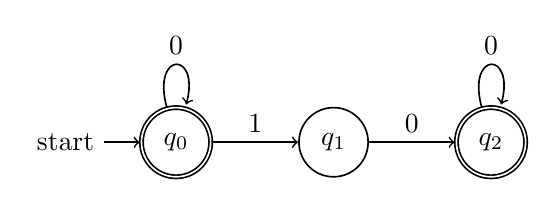
\begin{tikzpicture}[auto,node distance=2cm,on grid,semithick]
    \node[state,initial,accepting] (q0)   {$q_0$};
    \node[state] (q1) [right=of q0] {$q_1$};
    \node[state,accepting] (q2) [right=of q1] {$q_2$};
    \path[->]
    (q0) edge [loop above] node {0} (q0)
         edge node {1} (q1)
    (q1) edge node {0} (q2)
    (q2) edge [loop above] node {0} (q2);
\end{tikzpicture}

% Diagram for 01* ∪ 10*11*
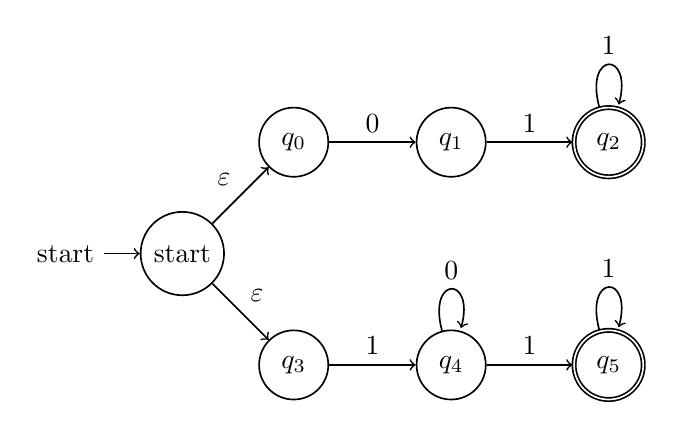
\begin{tikzpicture}[auto,node distance=2cm,on grid,semithick]
    \node[state,initial] (s)   {start};
    \node[state] (q0) [above right=of s] {$q_0$};
    \node[state] (q1) [right=of q0] {$q_1$};
    \node[state,accepting] (q2) [right=of q1] {$q_2$};
    \node[state] (q3) [below right=of s] {$q_3$};
    \node[state] (q4) [right=of q3] {$q_4$};
    \node[state,accepting] (q5) [right=of q4] {$q_5$};
    \path[->]
    (s) edge node {$\varepsilon$} (q0)
        edge node {$\varepsilon$} (q3)
    (q0) edge node {0} (q1)
    (q1) edge node {1} (q2)
    (q2) edge [loop above] node {1} (q2)
    (q3) edge node {1} (q4)
    (q4) edge [loop above] node {0} (q4)
         edge node {1} (q5)
    (q5) edge [loop above] node {1} (q5);
\end{tikzpicture}

% Diagram for 0(1 ∪ 0)*
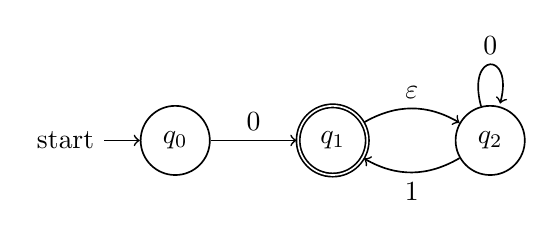
\begin{tikzpicture}[auto,node distance=2cm,on grid,semithick]
    \node[state,initial] (q0)   {$q_0$};
    \node[state,accepting] (q1) [right=of q0] {$q_1$};
    \node[state] (q2) [right=of q1] {$q_2$};
    \path[->]
    (q0) edge node {0} (q1)
    (q1) edge [bend left] node {$\varepsilon$} (q2)
    (q2) edge [bend left] node {1} (q1)
    (q2) edge [loop above] node {0} (q2);
\end{tikzpicture}

\end{document}
